\chapter{Referencial Teórico}
\label{sec:referencialteorico}

Este capítulo apresenta o referencial teórico sobre Teste de Software, Processos de Teste mais consolidados e algumas técnicas reconhecidas e utilizadas amplamente pela Comunidade Acadêmica e Indústria.

Serão apresentados na seção \ref{sec:processotestedesoftware} os conceito sobre os processos de teste prescritivos e ágeis, tomando como referencial alguns processos mais conhecidos na acadêmia.

Na seção \ref{sec:devops} apresentados conceitos e uma visão prática sobre DevOps e sua importância.

A subseção \ref{sec:revisaoliteraturacap2} é apresentado uma revisão da literatura, utilizando algumas técnicas de revisão sistemática.

Na seção \ref{sec:planejamentodapesquisa} é explanado toda a sistemática para realização da pesquisa do referencial teórico utilizado para este trabalho, bem como, strings de busca utilizadas, fontes de pesquisa e critérios de seleção dos estudos.

A subseção \ref{sec:identificacaodosestudos} mostra os passos necessários para a identificação dos estudos. Enquanto que na seção \ref{sec:selecaodosestudos} os estudos selecionados são exibidos, após sofrer os critérios de inclusão e exclusão.

Através dos resultados obtidos nas pesquisas, os trabalhos selecionados são discutidos na seção \ref{sec:discussoes}. Por fim, a conclusão deste capítulo é exposta na seção \ref{sec:conclusoescap2}.


\section{Processo de Teste software}
\label{sec:processotestedesoftware}

É uma atividade sistemática aplicada durante a integração da estrutura do programa visando a descobrir erros associados as interfaces entre os módulos. De acordo com Myers \cite{myers2004}, o principal objetivo do teste de software é revelar a presença de erros no produto. Atividade bastante efetiva em evidenciar a presença de defeitos de software. Sendo assim, um teste bem sucedido é aquele que consegue determinar casos de teste para os quais o programa em teste falhe.

O processo de teste de software consiste em uma analise dinâmica do produto, identificando e eliminando erros que persistem. O teste de produtos de software envolve basicamente quatro etapas:

\begin{itemize}
    \item Planejamento de testes;
    \item Projeto de casos de teste;
    \item Execução e avaliação dos resultados dos testes;
    \item Relato de erros.
\end{itemize}

\subsection{Processos Prescritivos}

Na história, o os softwares foram desenvolvidos de forma prescritiva, utilizando-se de práticas de desenvolvimento de software semelhantes a outras atividades de áreas como a engenharia civil \cite{BRAGA2015}. Nestas áreas inicialmente é definido um conjunto específico de ações, atividades e tarefas definidas em fases de forma sequencial e linear. Alguns modelos prescritivos são citados em Pressman \cite{PRESSMAN2011} como o modelo em cascata (Figura \ref{fig:figure21}) e modelos incrementais (Figura \ref{fig:figure22}), onde as características principais são o sequenciamento das fases. As fases de um modelo tradicional costumam seguir a sequencia composta por definição de requisitos, projeto do software, implementação, testes, integração, operação e manutenção.

\begin{figure}[!ht]
\centering
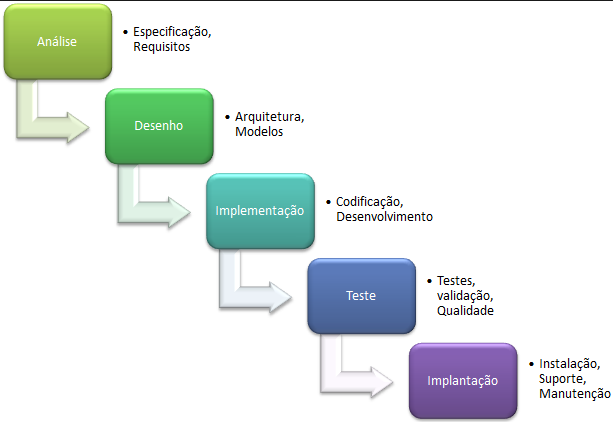
\includegraphics[width=.75\textwidth]{fig/figura21.png}
\caption{Exemplo de Modelo de Processo Cascata. (Fonte: Internet)}
\label{fig:figure21}
\end{figure}


\begin{figure}[!ht]
\centering
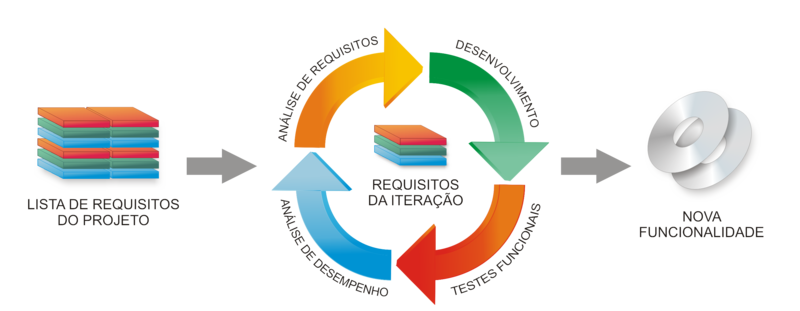
\includegraphics[width=.75\textwidth]{fig/figura22.png}
\caption{Exemplo de Modelo de Processo incremental. (Fonte: Internet)}
\label{fig:figure22}
\end{figure}

Em modelos tradicionais de desenvolvimento de software, a equipe de qualidade trabalham em de forma independente e muitas vezes em salas diferentes, aguardando a finalização do trabalho dos desenvolvedores para começarem a iniciar a etapa de testes (verificação e validação) no software. 
Após a realização dos testes, correção de possíveis \textit{bugs} e retestes, o software estará prestes a ser distribuído para os clientes, ou seja, estará em produção. Atividade essa desempenhada pela equipe de suporte, migração ou \textit{sysadmin} da organização.

Segundo Huttermann \cite{huttermann2012}, este modelo de trabalho com equipes separados gera barreiras como a ausência de uma padronização, pois, "\textit{uma vez que cada time desenvolve idioma próprio trabalhando em seus problemas individualmente e não em prol de um único objetivo.}" 

\subsection{Processo Ágil}

Com a necessidade cada vez maior do mercado consumidor de software, existe uma necessidade muito grande do mercado para que as empresas criem valor para os seus clientes através de software. Portando a entrega do software se tornou um dos grandes desafios das organizações, com a premissa de que software pronto é software em produção. Diante disso, e da necessidade de entrega de valor aos seus clientes os \textit{gaps} entre requisito, codificação, teste e entregam precisaram ser reduzidos. As organizações descobriram que os modelos tradicionais de desenvolvimento de software e de entrega não são suficientes. Os processos manuais são propensos a erros, quebras, desperdício e atraso de resposta às necessidades de negócios \cite{BRAGA2015}. Com a automatização de tarefas, criação de equipes multitarefas, e forma de trabalho holística as organizações podem focar no que realmente é importante: A entrega de valor aos seus clientes. Ao contrário de um modelo de desenvolvimento burocrático, sequencial e orientado à contratos as organizações tem se atentado que é importante a automatização de tarefas e entrega (mesmo que parciais) de valor aos seus clientes.

As metodologias tradicionais traziam um desenvolvimento de software pautado em estágios sequenciais e lineares, e são atualmente denominadas metodologias pesadas ou orientadas a documentação, porque cada o término de cada etapa é associado a uma documentação padrão que deve ser aprovada e assim poderá ser iniciada uma nova etapa \cite{ROYCE1970}. Nestas metodologias toda a responsabilidade por identificar \textit{bugs} é da equipe de qualidade, e o software não chega até o cliente até que a equipe de qualidade valide, a equipe de administração de redes, baco de dados e sistemas prepare o ambiente e por fim, a equipe de operação prepare o sistema para produção. Consequentemente os erros são encontrados tardiamente, os requisitos poderão não mais satisfazer as necessidades do negócio, e mais caro ficará o para corrigir e desenvolver novas soluções \cite{PRESSMAN2011}.

Inspirado em resolver as dificuldade proporcionada pela metodologia tradicional de desenvolvimento de software nasceu, na década de 90, o movimento ágil, que teve como principal objetivo que a equipe de desenvolvimento de software respondesse de forma mais dinâmica às constantes mudanças do negócio. Foi então estabelecido o Manifesto Ágil \cite{Beck2001}, visando priorizar os \textit{indivíduos, software executável, colaboração com o cliente, respostas rápidas a mudanças}, interações a processos e ferramentas e negociação de contratos.

No contexto das metologias ágeis várias possíveis e prováveis divergências entre o negócio e o produto se tornaram mais fáceis de serem resolvidas através de técnicas de aproximação do cliente à equipe de desenvolvimento, proporcionando integração contínua, reuniões diárias e times pequenos porém multifuncionais. Após a fase de aceitação e adaptação das empresas às metodologias ágeis de desenvolvimento, os desenvolvedores, testadores e demais membros da equipe do projeto se agruparam em prol do objetivo de desenvolver software ágil que respondessem às necessidades do negócio. Porém, ainda nesse novo contexto, a equipe de operação continuou isolada trabalhando como um time a parte, recebendo os \textit{builds}, integrando-os e os colocando em produção. E elas estão sendo cada vez mais aceitas pielas organizações, pois estas vem descobrindo que os modelos tradicionais de desenvolvimento de software e de entrega não são suficientes. Os processos manuais são propensos a erros, quebras, desperdício e atraso de resposta às necessidades de negócios \cite{WOOTTON2013}. Como visto na figura \ref{fig:figure23} em um processo Ágil a organização está orientada à entrega do produto, neste caso as entregas parciais são realizadas em curtos prazos de tempo para que os clientes possam validar os resultados e o desenvolvimento do software esteja alinhado ao negócio.


\begin{figure}[H]
\centering
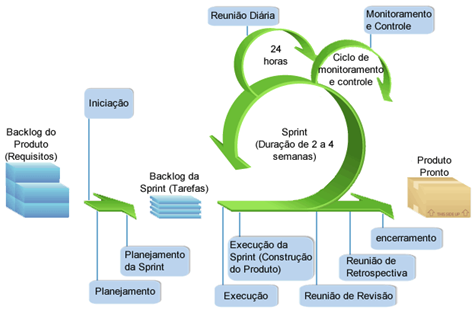
\includegraphics[width=.75\textwidth]{fig/figura23.png}
\caption{Exemplo de Modelo de Processo Ágil. (Fonte: Internet)}
\label{fig:figure23}
\end{figure}

\section{DevOps}
\label{sec:devops}

O Termo DevOps teve sua origem em 2008 quando \textit{Patrick Debois} publicou um artigo intitulado "\textit{Agile and Operations Infrastrucuture: How Infra-gile Are You?}" \cite{Debois2008}. Onde demonstrava que a infraestrutura poderia também responder de forma ágil à mudanças de negócios, se adaptando e respondendo constantemente. Neste ano, durante uma conferência sobre práticas ágeis houve a apresentação "\textit{Agile Infrastructure}" de Debois e \textit{Andrew Shafer}, onde também foi criada a lista \textit{agile-sysadmin} na Europa focada na discussão de metodologias ágeis na infraestrutura. A partir desta lista, vários estudos e conferências surgiram, popularizando o termo. Até que em 2009 hove a conferência \textit{Velocity da O’Reilly} onde foi apresentado o trabalho "\textit{10+ Deploys Per Day: Dev and Ops Cooperation at Flickr}" por  John Allspaw e Paul Hammond demonstrando o estudo de caso sobre a implantação em uma empresa onde havia a prática da colaboração entre as equipes de desenvolvimento e operação em atendimento à dinâmica do mercado \cite{ALLSPAW2009}. A partir deste evento surgiu a ideia de criar um novo evento, o DevOpsDays, realizados em diversos países, a partir de iniciativas locais, disseminando essa nova cultura.

Atualmente o termo DevOps é muito amplo, envolve inúmeras atividades e aspectos, como a automação, medição e o compartilhamento de conhecimentos \cite{huttermann2012} e pode se referir a qualquer prática que inova a interação entre desenvolvimento e operações. É uma abordagem baseada em princípios \textit{Lean} e Ágil \cite{BRAGA2015}. De tal maneira, que permite a Organização focar esforços no produto/cliente de maneira rápida, eficiente, de maneira contínua e com \textit{feedbacks} mais rápidos, onde, toda a equipe de desenvolvimento, qualidade e operação trabalha de forma colaborativa e simbiótica. Na figura \ref{fig:figure24} é possível entender o funcionamento de um modelo de processo que utiliza DevOps, no qual uma quantidade grande de atividades corriqueiras são criadas e a integração entre operação, teste e desenvolvimento ocorre o tempo todo de forma automatizada.

\begin{figure}[H]
\centering
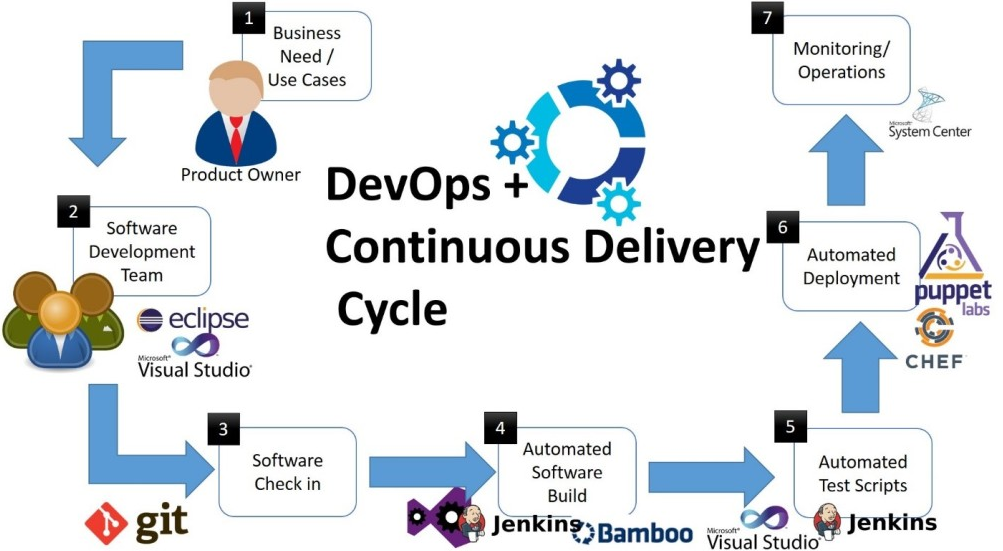
\includegraphics[width=.75\textwidth]{fig/figura24.png}
\caption{Exemplo de Modelo de Processo que utiliza DevOps. (Fonte: Internet)}
\label{fig:figure24}
\end{figure}

Em resumo, segundo Braga \cite{BRAGA2015} o DevOps é um movimento cultural, focado na colaboração e do compartilhamento de conhecimentos entre as equipes. A Organização pode possuir processos e ferramentas automatizadas eficientes, contudo se torna inútil senão utilizada corretamente. 
Por fim, construir uma cultura pautada nos objetivos da Organização ao invés dos objetivos da equipe separada é o que o DevOps preconiza.

\section{Revisão da Literatura}
\label{sec:revisaoliteraturacap2}

Esta sessão apresenta uma revisão da literatura sobre quais são os processos, métodos, e \textit{frameworks} de teste existentes no ponto de vista acadêmico e da indústria. Esta pesquisa incide sobre os artigos científicos publicados nos últimos cinco anos, a partir de janeiro de 2010 a dezembro de 2015.

Elenca-se que apesar de se utilizar algumas ferramentas da revisão sistemática, este estudo não visa realizar uma revisão sistemática, e sim, recuperar resultados efetivos das máquinas de busca mais conhecidas, aplicando expressões e filtros de datas e idiomas no qual as pesquisas foram escritas. 

O principal objetivo desta revisão da literatura foi buscar pesquisas relacionadas à processos de uso especifico para o Teste de Software, uso de DevOps e Métodos Ágeis. Preferencialmente trabalhos com estudo de caso e aplicações na indústria foram selecionados, com o intuito de enriquecer mais ainda essa pesquisa. Para nortear a pesquisa, foram concebidas as seguintes questões:

\begin{itemize}
\item Q01 - Existem na literatura trabalhos de revisões sistemáticas sobre processos de teste de software?   
\item Q02 - Quais são os processos, métodos e \textit{frameworks} de testes de software desenvolvidos nos últimos cinco anos?
\item Q03 - Quais trabalhos estão aplicando DevOps e Métodos Ágeis em processo de teste?
\end{itemize}

Com o intuito de realizar uma busca e classificação da pesquisa com o propósito de responder as questões Q01, Q02 e Q03, cada referência incluída nesta revisão foi agrupada em dissertações e teses, métodos e processos já consolidados e artigos científicos. Ao final as análises realizadas foram objetivas, neste caso são extraídos diretamente dos estudos ou conhecimentos que foram obtidos por meio de conclusões e analises do revisor.

Assim sendo, as pesquisas extraídas da revisão foram agrupadas da seguinte maneira:

\begin{itemize}
\item Teses e dissertações relacionadas à processos de teste;
\item Artigos científicos sobre processos de teste, \textit{frameworks} de processo;
\item Artigos que abordem revisões sistemáticas sobre processos de teste;
\item Processos e modelos de processos de teste já reconhecidos.
\end{itemize}

Os artigos, teses e dissertações foram selecionadas quando seus resumos e palavras chaves estavam visíveis durante a execução do protocolo ou disponibilizadas por meio de uma leitura criteriosa para encontrar fontes que apoiassem fortemente a pesquisa. Por exemplo, trabalhos escritos em idiomas que não fossem em inglês e português, que não continham informações de resumo, titulo e palavras chaves aderentes à pesquisa foram descartados. Por fim, foram selecionados trabalhos que trouxessem informações relevantes sobre processos de uso específico para o teste de software, trabalhos que fomentassem a aplicação e estudos de caso.

Nas subseções seguintes, são abordadas de forma detalhada a metodologia utilizada para o planejamento, identificação e seleção dos resultados encontrados na revisão da literatura.

\section{Planejamento da Pesquisa}
\label{sec:planejamentodapesquisa}

Nesta seção são abordados a construção do protocolo de pesquisa, a seleção das fontes e os critérios de seleção dos estudos identificados na literatura.

\subsection{\textit{Strings} de busca}
\label{sec:stringdebusca}

Para direcionar as buscas das evidências existentes na literatura, considerando as questões da pesquisa, foram definidas algumas palavras chaves para a elaboração de um protocolo adaptado para cada máquina de busca. A seguir a \textit{string} de busca criada e utilizada para cada máquina de busca respectivamente.

\begin{itemize}
\item P1 - \textit{String} em Inglês - (((Title:"Software Testing" OR Title:"Testing Engineering" OR Abstract:"Software Testing" OR Abstract:"Testing Engineering") AND (Title:Process OR Title:Framework OR Title:Method OR Title:Agile OR Title:Devops) AND (Abstract:Process OR Abstract:Framework OR Abstract:Method OR Abstract:Agile OR Abstract:Devops)))
\item P2 - \textit{String} em Português -  (Todos os campos:Teste de Software) E (Todos os campos:Processo OU Todos os campos:Arcabouço OU Todos os campos:Metódo OU Todos os campos:Ágil OU Todos os campos:Devops)
\end{itemize}

\subsection{Fontes da Pesquisa}
\label{sec:fontesdapesquisa}

A pesquisa foi realizada entre janeiro de 2010 a dezembro de 2015, em idioma português (quando possível) e inglês, incidindo-se nas seguintes bases:

\begin{itemize}
\item IEEE Xplore Digital Library;
\item ACM;
\item Web of Science;
\item BDTD - Biblioteca Digital Brasileira de Teses e Dissertações.
\end{itemize}

As buscas foram configuradas para trazer os resultados dos artigos em Língua Inglesa por ser a língua padrão para publicações internacionais. Exceto pela fonte de dados BDTD, pois o enfoque foi encontrar teses e dissertações nacionais.

\subsection{Critérios de seleção dos estudos}
\label{sec:criteriosdeselecao}

Após a construção do protocolo e a escolha das máquinas de busca que fomentaram a pesquisa, os resultados obtidos foram analisados afim de evidenciar a sua relevância. Por fim, os critérios de seleção utilizados foram os seguintes.

\begin{enumerate}
\item [i] Trabalhos com aplicação prática e/ou estudo de caso na indústria;
\item [ii] Trabalhos com ou sem estudo de caso voltadas para micro e pequenas empresas;
\item [iii] Revisões sistemáticas sobre processos de teste;
\item [iv] Processos e modelos de processo já conhecidos pela comunidade acadêmica e indústria.
\end{enumerate} 

Alguns critérios de exclusão também foram definidos afim de alinhar os resultados encontrados com a finalidade desta pesquisa.

\begin{enumerate} 
    \item [i] Artigos científicos que não abordam processos/métodos/\textit{frameworks} de teste de software;
    \item [ii] Pesquisas que não contenham estudos de caso e aplicações práticas;
\end{enumerate}

\section{Identificação dos Estudos}
\label{sec:identificacaodosestudos}

A busca foi dividida em duas partes. Sendo a primeira parte a execução da \textit{string} nas máquinas de busca  em inglês, focadas para artigos científicos, a segunda etapa foi busca por dissertações e teses nacionais.

\subsection{Primeira Execução}
\label{sec:primeiraexecucao}

Após a definição das \textit{strings} de busca na subseção \ref{sec:stringdebusca}, realizou-se a execução do protocolo P1 separando-o por fonte de pesquisa (subseção \ref{sec:fontesdapesquisa}). 

Executando-se o protocolo P1 na primeira rodada, foram retornados 506 referências, das quais 112 artigos são oriundos da base \textit{IEEE Xplore Digital Library}, 20 foram da base da \textit{ACM}, 374 da \textit{Web of Sicience}. A figura \ref{fig:figure31} mostra o gráfico com o percentual de resultados encontrados para cada fonte de pesquisa.

\begin{figure}[!ht]
\centering
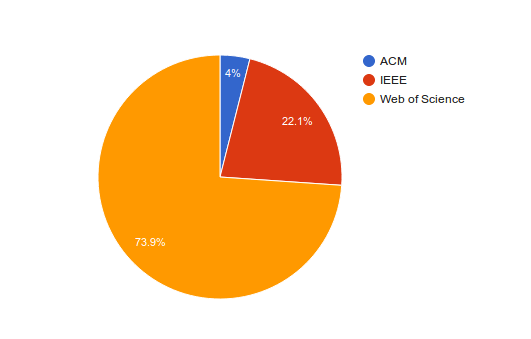
\includegraphics[width=1\textwidth]{fig/figura31.png}
\caption{Percentual dos resultados da execução do protocolo P1 por fonte de pesquisa.}
\label{fig:figure31}
\end{figure}

\subsection{Segunda Execução}

Na segunda execução, o objetivo foi buscar por teses e dissertações na Biblioteca Digital Brasileira de Teses e Dissertações (BDTD), que apresentassem pesquisas relacionadas a criação e aplicação  de processos de teste de software no contexto da indústria. Pesquisas, relacionadas à métodos ágeis e DevOps com aplicação prática mercado também foram considerados.

Para a segunda execução foram retornados 1126 referências, todas elas, teses e dissertações nos últimos cinco anos. 

\section{Seleção dos Estudos}
\label{sec:selecaodosestudos}

Na seleção dos estudos o objetivo é realizar uma categorização primária das pesquisas encontradas por meio da aplicação dos critérios de inclusão e exclusão definidos na subseção \ref{sec:criteriosdeselecao}. Essa categorização primária incidiu sob os resultados finais da primeira e segunda execução. A Tabela \ref{tab:3.1} apresenta o resultado quantitativo da identificação dos estudos (subseção \ref{sec:identificacaodosestudos}) realizado pelos protocolos P1 e P2.

\begin{table}[H]
\centering
\caption{Total de artigos, teses e dissertações identificados na pesquisa.}
\label{tab:3.1}
  \scalebox{0.75}{
\begin{tabular}{|c|c|c|c|c|}
\hline
\textbf{ACM} & \textbf{IEE} & \textbf{Web of Science} & \textbf{BDTD} & \textbf{Total} \\ \hline
20           & 112          & 374                     & 1126          & 1632           \\ \hline
\end{tabular}
}
\end{table}

Com a soma dos resultados encontrados na execução dos protocolos P1 e P2, total de 1632 (mil seiscentos e trinta e dois) artigos, foram analisados os resultados aplicando os critérios de inclusão e exclusão descrito na subseção \ref{sec:criteriosdeselecao}. Mais três categorias foram criadas para a realização da classificação dos resultados:

\begin{itemize}
\item [i] Artigos duplicados;
\item [ii] Artigos descartados (usando os critérios de exclusão);
\item [iv] Artigos aceitos (usando os critérios de inclusão).
\end{itemize}

As análises dos artigos foram realizadas sobe os resultados das máquinas de busca (Subseção \ref{sec:fontesdapesquisa}), neste caso, a cada execução foi selecionado um conjunto de trabalhos. A seleção foi realizada por uma leitura criteriosa do conteúdo dos resumos, títulos e palavras chaves dos artigos. Em alguns casos artigos exigiram uma leitura mais profunda afim de encontrar alguns dos aspectos definidos nos critérios de classificação.

\subsection{Exclusão de Estudos}
\label{sec:exclusaoestudos}

Artigos que se encaixavam nos critérios de exclusão (subseção \ref{sec:criteriosdeselecao}) ou duplicados foram excluídos desse estudo. Basicamente trabalhos relacionados à processos de teste sem estudo de caso e análise prática, artigos sobre DevOps e Métodos Ágeis com finalidades especificas e sem contexto da indústria ou conhecimento empírico também foram excluídos.

Em síntese os trabalhos examinados que não atendiam os critérios de seleção (subseção \ref{sec:criteriosdeselecao}) e que estavam nesse padrão, foram excluídos:

\begin{itemize}
\item Estudo científicos que abordam apenas processos de teste de software fora do contexto prático da indústria;
\item Estudo científicos que abordam processos de teste de software para uso especifico, como sistemas aviônicos, embarcados e críticos;
\item Estudo científicos que não abordam assuntos de teste de software;
\end{itemize}

\subsection{Estudos Aceitos}
\label{sec:estudosaceitos}
Os estudos aceitos neste trabalho adotaram o mesmo método de análise aplicado na subseção \ref{sec:criteriosdeselecao}. Foram utilizados os seguintes critérios de inclusão para realização das analises e classificações:

\begin{itemize}
\item Trabalhos com aplicação prática e/ou estudo de caso na indústria;
\item Trabalhos com ou sem estudo de caso voltadas para micro e pequenas empresas;
\item Revisões sistemáticas sobre processos de teste;
\item Processos  e  modelos  de  processo  já  conhecidos  pela  comunidade  acadêmica  e
indústria.
\end{itemize}

Após a realização das análises e agrupamento dos estudos em, teses e dissertações, artigos científicos, revisões sistemáticas e por fim processos de teste reconhecidos e mais citados nos trabalhos examinados, a tabela \ref{tab:3.2} foi criada listando os principais estudos que nortearam esse trabalho.

\begin{table*}[ht]
\centering
\caption{Quantitativo dos principais trabalhos aceitos para essa pesquisa.}
\label{tab:3.2}
  \scalebox{0.75}{
\begin{tabular}{|c|c|c|c|c|c|c|c|}
\hline \textbf{Teses e Dissertações } &\textbf{Revisões Sistemáticas} &\textbf{Artigos Científicos} &\textbf{Processos de Teste} \\ 
\hline 4 &2 &18 &6\\
\hline 
\end{tabular} 
}
\end{table*}

As discussões e trabalhos relacionados sobre os estudos selecionados serão melhor argumentados no item \ref{sec:discussoes}. Para facilitar o entendimento os estudos aceitos foram divididos de acordo com as categorias da tabela \ref{tab:3.2}.

\section{Discussões e Trabalhos Relacionados}
\label{sec:discussoes}

Os estudos aceitos e listados no item \ref{sec:estudosaceitos} serviram de embasamento principal para essa pesquisa e evidenciam o enfoque desse trabalho. As discussões realizadas aqui foram divididas pela categorização dos resultados da pesquisa como supramencionado no item anterior. Neste caso teses e dissertações, revisões sistemáticas, artigos científicos e processos de teste já reconhecidos pela comunidade acadêmica e da indústria.

\subsection{Teses e dissertações}
\label{sec:tesesdissertacoes}

O trabalho criação do arcabouço \textbf{KITest: Um arcabouço de conhecimento e melhoria de processo de teste} \cite{Nina2011} que funciona como um conjunto de ferramentas e técnicas "para agregar o conhecimento em teste e disponibilizá-lo para a comunidade com a intenção de facilitar a sua transferência, a definição e a melhoria de processos de teste, com mais qualidade". 

Com aplicação do conhecimento abordado na pesquisa, a ferramenta KITTool foi criada com a intenção de auxiliar no diagnóstico de processos e orientar possíveis melhorias. Um processo genérico foi modelado baseado nas práticas do TMMi em formato de mapa mental, denominado KITMap.

O objetivo principal do arcabouço KITest (\textit{Knowledge and Improvement on Test}) é visto abaixo:

\begin{itemize}
\item Ter um módulo na criação do arcabouço KITest (\textit{Knowledge and Improvement on Test}) que funciona como um conjunto de ferramentas e técnicas "para agregar o conhecimento em teste e disponibilizá-lo para a comunidade com a intenção de facilitar a sua transferência, a definição e a melhoria de processos de teste, com mais qualidade".
\item Como aplicação do conhecimento abordado na pesquisa, a ferramenta KITTool foi criada com a intenção de auxiliar no diagnóstico de processos e orientar possíveis melhorias. Um processo genérico foi modelado baseado nas práticas do TMMi em formato de mapa mental, denominado KITMap.
\item Permitisse a centralização das informações sobre a atividade de teste, de uma maneira organizada, para facilitar a compreensão e a aquisição do conhecimento em teste;
\item Ter um módulo que viabilizasse a interação da comunidade com o módulo de conhecimento em teste, de forma que a comunidade fosse capaz de aplicar esse conhecimento na definição de um processo de teste com qualidade, seguindo as premissas de qualidade do TMMi, que concentra as melhores práticas existentes nessa área; e
\item Possuir um mecanismo que ajude a constante evolução desse conhecimento sobre teste, de forma que essa evolução fosse fundamentada na realimentação da comunidade, com base nos relatos de experiência sobre o uso das informações organizadas no módulo.
\end{itemize}

Conclui-se que a proposta do arcabouço KiTest é interessante no ponto de vista de disseminação de conhecimento em teste de software e uma ferramenta para nortear empresas/instituições de T.I. a alcançarem a maturidade desejada em seus Processos de Teste. Embora segundo a própria autora é necessário a aplicação e validação prática do arcabouço, nos estudos realizados dentro de uma experimentação controlada os resultados foram satisfatórios. Por fim, o arcabouço lida mais com aquisição de conhecimento em teste de software, avaliação do processo de teste de instituições da T.I., fazendo-se necessário da existência de pesquisas que auxiliem não somente no alinhamento da maturidade da empresa, como também pesquisas que corroborem a implantação das áreas de processo necessárias para se alcançar tais níveis de maturidade.

No trabalho \textbf{Um Arcabouço para Avaliação do Nível de Maturidade em Teste de Software para Micro e Pequenas Empresas} \cite{Araujo2013}, que apresenta um arcabouço validado na indústria para avaliação do nível de maturidade dos processos de teste das Micro e Pequenas Empresas com base nas boas práticas do TMMI. 

O autor utilizou da ajuda de questionários aplicados em diversas Micro e Pequenas Empresas do estado de Goiás para coletar dados inerentes à maturidade do processo de teste das empresas. Segundo o autor, o questionário evidenciou a carência das empresas do referido estado no sentido de boas práticas para o processo de teste. Todavia a pesquisa além de colaborar com uma métrica de maturidade dentro panorama do mercado de T.I pesquisado, ajudou a mostrar para as empresas a necessidade de melhorias.

A pesquisa \textbf{Melhoria do Processo de Teste para as Micro e Pequenas Empresas Brasileiras} \cite{SilvaDias2015} compara os processos de teste existentes na indústria brasileira e propõe melhorias do ponto de vista dos estudos realizados. 
A autora realiza comparações com iniciativas nacionais, como o Método FreeTest e MPT.Br para propor um modelo de maturidade considerando as limitações das micro e pequenas empresas de desenvolvimento de software, e uma abordagem para implementar os processos de teste definidos nesse modelo.

Apesar do levantamento \textit{in-loco} das informações de maturidade dos processos de teste de software das empresas e as propostas de melhoria para um processo, não houve validação prática do estudo. 

Outro estudo que corroborou substancialmente este trabalho foi o \textbf{Um Panorama Sobre o Uso de Práticas DevOps nas Indústrias de Software} \cite{BRAGA2015}, no qual o autor realiza um mapeamento sistemático do uso de práticas de DevOps na indústria. O autor elicita as práticas mais comuns utilizadas pelas empresas, realiza uma pesquisa utilizando questionários no mercado brasileiro de T.I. e como propostas de trabalhos futuros evidência a importância da criação de um processo de desenvolvimento que utilize práticas específicas de DevOps como um nicho de pesquisa.

\subsection{Processos de Teste MPT.Br e FreeTest}
\label{processosteste}

Processos são definidos por ações, observações e tomadas de decisões com a finalidade de obter um produto final como saída, sendo que, essas ações podem ocorrer em paralelo ou de forma sequencial. Processos de software agrega atividades, métodos bem como, as práticas utilizadas no desenvolvimento de um produto de software.

Para corroborar essa pesquisa os processos MPT.Br \cite{GuiaMPTbr} e o Método FreeTest \cite{Camilo-junior2012} foram analisados. Um processo bem definido e gerenciável permite que métricas e projetos de teste sejam facilmente alcançados com sucesso, a replicabilidade do processo é outro fator muito importante, pois é imprescindível que com um mesmo processo diferentes tipos de projetos possam ser executados. Com a análise dos dois processos e as inferências dos outros estudos avaliados pretende-se promover a melhoria do processo contido no Método FreeTest.

\subsection{MPT.Br}

O MPT.Br (Melhoria do Processo de Teste Brasileiro) \cite{GuiaMPTbr} foi concebido a fim de apoiar as organizações através de elementos essenciais da disciplina de teste. O MPT.Br como alguns outros processos de desenvolvimento de software nacionais foram inspirados no MPS.Br \cite{Softex} que por sua vez se inspirou no Modelo de Processo CMMI \cite{cmmi}. O MPT.Br aborda as melhores práticas envolvidas nas atividades inerentes à fase de teste de software de uma organização. Seu foco principal está em:

\begin{itemize}
    \item Ser um modelo de referência para a definição/implantação e melhoria do processo de teste das organizações;
    \item Melhoria contínua dos processos e aumento do nível de maturidade da empresa de acordo com suas necessidades;
    \item Boas práticas a serem empregadas ao longo da implementação do processo na organização. Sua divisão em Áreas de Processos, Atividades Especificas e práticas Genéricas contribuem para a implantação do processo.
\end{itemize}

O MPT.Br também foi concebido com base em modelos de referência em teste de software como, \textit{Testability Support Model (TSM)}, o \textit{Testing Maturity Model (TMM)}, a \textit{Test Process Improvement (TPI)}, a \textit{Test Organization Maturity (TOMtm)}, o \textit{Testing Assessement Program (TAP)}, o \textit{Testing Improvement Model (TIM)}, o \textit{Testing Maturity Model Integration (TMMI)}, o \textit{Maturity Model for Automated Software Testing}, o Modelo de Melhoria de Teste (MMT).

O MPT.Br é dividido em Áreas de Processo (AP), Práticas Especificas e Práticas Genéricas. Na tabela \ref{tab:3.3} pode ser visto tais itens dentro de seus respectivos níveis de maturidade.

\begin{table}[H]
\centering
\caption{Estrutura do MPT.Br \cite{GuiaMPTbr}.}
\label{tab:3.3}
  \scalebox{0.75}{
    \begin{tabular}{|l|l|l|l|}
    \hline
    \multicolumn{1}{|c|}{Nível de Maturidade} & \multicolumn{1}{c|}{Áreas de Processo} & \multicolumn{1}{c|}{Práticas Especificas} & \multicolumn{1}{c|}{Práticas Genéricas} \\ 
    \hline
    \multicolumn{1}{|c|}{Nível 1} & \multicolumn{1}{c|}{GPT} & \multicolumn{1}{c|}{GPT1 a GPT20} & \multicolumn{1}{c|}{PG1 a PG6} \\ 
    \cline{2-3}
    \multicolumn{1}{|c|}{} & \multicolumn{1}{c|}{PET} & \multicolumn{1}{c|}{PET1 a PET4} & \multicolumn{1}{c|}{} \\ 
    \hline
    \multicolumn{1}{|c|}{Nível 2} & \multicolumn{1}{c|}{GRT} & \multicolumn{1}{c|}{GRT1 a GRT5} & \multicolumn{1}{c|}{PG7 a PG9} \\ 
    \cline{2-3}
    \multicolumn{1}{|c|}{} & \multicolumn{1}{c|}{GRT} & \multicolumn{1}{c|}{GPT21 a GPT25} & \multicolumn{1}{c|}{} \\ 
    \cline{2-3}
    \multicolumn{1}{|c|}{} & \multicolumn{1}{c|}{PET} & \multicolumn{1}{c|}{PET5 a PET6} & \multicolumn{1}{c|}{} \\ 
    \hline
    \multicolumn{1}{|c|}{Nível 3} & \multicolumn{1}{c|}{FDT} & \multicolumn{1}{c|}{FDT1 a FDT4} & \multicolumn{1}{c|}{} \\ 
    \cline{2-3}
    \multicolumn{1}{|c|}{} & \multicolumn{1}{c|}{GDQ} & \multicolumn{1}{c|}{GDQ1 a GDQ3} & \multicolumn{1}{c|}{} \\ 
    \cline{2-3}
    \multicolumn{1}{|c|}{} & \multicolumn{1}{c|}{MAT} & \multicolumn{1}{c|}{MAT1 a MAT5} & \multicolumn{1}{c|}{} \\ 
    \cline{2-3}
    \multicolumn{1}{|c|}{} & \multicolumn{1}{c|}{OGT} & \multicolumn{1}{c|}{OGT1 a OGT10} & \multicolumn{1}{c|}{} \\ 
    \cline{2-3}
    \multicolumn{1}{|c|}{} & \multicolumn{1}{c|}{TDA} & \multicolumn{1}{c|}{TDA1 a TDA7} & \multicolumn{1}{c|}{} \\ 
    \cline{2-3}
    \multicolumn{1}{|c|}{} & \multicolumn{1}{c|}{TES} & \multicolumn{1}{c|}{TES1 a TES5} & \multicolumn{1}{c|}{} \\ 
    \cline{2-3}
    \multicolumn{1}{|c|}{} & \multicolumn{1}{c|}{TRE} & \multicolumn{1}{c|}{TRE1 a TRE4} & \multicolumn{1}{c|}{} \\ 
    \cline{2-3}
    \multicolumn{1}{|c|}{} & \multicolumn{1}{c|}{GPT} & \multicolumn{1}{c|}{GPT26 a GPT28} & \multicolumn{1}{c|}{} \\ 
    \cline{2-3}
    \multicolumn{1}{|c|}{} & \multicolumn{1}{c|}{PET} & \multicolumn{1}{c|}{GPT26 a GPT28} & \multicolumn{1}{c|}{} \\ 
    \hline
    \multicolumn{1}{|c|}{Nível 4} & \multicolumn{1}{c|}{AQP} & \multicolumn{1}{c|}{AQP1 a AQP5} & \multicolumn{1}{c|}{} \\ 
    \cline{2-3}
    \multicolumn{1}{|c|}{} & \multicolumn{1}{c|}{GDD} & \multicolumn{1}{c|}{GDD1 a GDD3} & \multicolumn{1}{c|}{} \\ 
    \cline{2-3}
    \multicolumn{1}{|c|}{} & \multicolumn{1}{c|}{TNF} & \multicolumn{1}{c|}{TNF1 a TNF3} & \multicolumn{1}{c|}{} \\ 
    \cline{2-3}
    \multicolumn{1}{|c|}{} & \multicolumn{1}{c|}{OGT} & \multicolumn{1}{c|}{OGT11 e OGT12} & \multicolumn{1}{c|}{} \\ 
    \hline
    \multicolumn{1}{|c|}{Nível 5} & \multicolumn{1}{c|}{AET} & \multicolumn{1}{c|}{AET1 a AET6} & \multicolumn{1}{c|}{} \\ 
    \cline{2-3}
    \multicolumn{1}{|c|}{} & \multicolumn{1}{c|}{CEP} & \multicolumn{1}{c|}{CEP1 a CEP5} & \multicolumn{1}{c|}{} \\ 
    \cline{2-3}
    \multicolumn{1}{|c|}{} & \multicolumn{1}{c|}{GDF} & \multicolumn{1}{c|}{GDF1 a GDF6} & \multicolumn{1}{c|}{} \\ 
    \hline
    \end{tabular}
}
\end{table}

A escolha do MPT.Br como base para essa pesquisa se dá pelo fato de que além de ser uma iniciativa nacional amplamente utilizada por Organizações e ser focado para o contexto de MPEs, o MPT.Br tem em sua estrutura dois componentes importantes: 

\begin{itemize}
    \item Modelo de Referência: Que apresenta a estrutura do processo, em áreas, práticas (especificas e genéricas) do nível de maturidade;
    \item Modelo de Avaliação: Aborda os critérios necessários para se avaliar um processo de teste de uma organização;
\end{itemize}

O MPT.Br possui um guia de Referência e de Avaliação que são de suma importância para guiar a empresa na implantação do processo de teste. Com a ajuda do Guia de Avaliação é possível que de tempos em tempos a Organização realiza avaliações de maturidade do seu processo e tome decisões para alcançar níveis mais altos ou ajustar alguma Área de Processo que não esteja como desejado. Apesar do MPT.Br ser proposto para organizações de todos os tamanhos e ser indicado para MPEs, o mesmo ainda possui muitas atividades que não estão totalmente alinhadas às necessidades de Organizações menores ou que desejam usar Métodos Ágeis. Logo nota-se uma oportunidade de melhoria, no refinamento da estrutura do Guia de Referência e também na necessidade de uma organização manter sempre seu processo em um nível de maturidade desejado.

\subsection{Método FreeTest}
\label{freetest}

O Método FreeTest \cite{Camilo-junior2012} surgiu como uma proposta completa para as Micro e Pequenas Empresas de T.I., pois desde a sua definição os autores do projeto se preocuparam com todas as necessidades que uma Organização teria, neste caso, um processo enxuto, ferramentas, técnicas e base de conhecimento para auxiliar as organizações à alcançarem o seu objetivo de maturidade. O projeto nasceu a partir do Estudo e Definição de Processo de Teste de Software para MPEs de TI, através do programa PAPPE Integração apoiado pela Fundação de Amparo à Pesquisa do Estado de Goiás (FAPEG)/Financiadora de Estudos e Projetos (FINEP) e, pelos pesquisadores do Instituto de Informática da Universidade Federal de Goiás (UFG) em conjunto com Organizações de T.I. do estado de Goiás \cite{Camilo-junior2012a}.

O FreeTest foi inspirado em modelos de maturidade como TMMI e MPT.Br. De forma geral o Método consiste em um conjunto de processos, ferramentas e conhecimento em teste de software que estabelece uma solução de fácil aplicação para MPEs que desejam ter um processo de teste definido e/ou melhorar seus processos e ferramentas. A estrutura do Método FreeTest é mostrado na tabela \ref{tab:3.4}.


\begin{table}[H]
\centering
\caption{Estrutura do Método FreeTest \cite{Camilo-junior2012}.}
\label{tab:3.4}
  \scalebox{0.75}{
    \begin{tabular}{|l|l|l|}
    \hline
    \multicolumn{1}{|c|}{Nível de Maturidade} & \multicolumn{1}{c|}{Áreas de Processo} & \multicolumn{1}{c|}{Práticas Específicas} \\ 
    \hline
    \multicolumn{1}{|c|}{Nível A} & \multicolumn{1}{c|}{TPE} & \multicolumn{1}{c|}{TPE1 a TPE4} \\ 
    \hline
    \multicolumn{1}{|c|}{Nível B} & \multicolumn{1}{c|}{INC} & \multicolumn{1}{c|}{INC1 a INC3} \\ 
    \hline
    \multicolumn{1}{|c|}{Nível C} & \multicolumn{1}{c|}{TRG} & \multicolumn{1}{c|}{TRG1 a TRG4} \\ 
    \hline
    \multicolumn{1}{|c|}{Nível D} & \multicolumn{1}{c|}{TDA} & \multicolumn{1}{c|}{TDA1 a TDA3} \\ 
    \cline{2-3}
    \multicolumn{1}{|c|}{} & \multicolumn{1}{c|}{TRQ} & \multicolumn{1}{c|}{TRQ1 a TRQ2} \\ 
    \hline
    \multicolumn{1}{|c|}{Nível E} & \multicolumn{1}{c|}{TFU} & \multicolumn{1}{c|}{TFU1 a TFU3} \\ 
    \cline{2-3}
    \multicolumn{1}{|c|}{} & \multicolumn{1}{c|}{GPT} & \multicolumn{1}{c|}{GPT1} \\ 
    \hline
    \end{tabular}
    }
\end{table}

Como já mencionado o diferencial do Método FreeTest é sua abordagem enxuta e sua concepção. Para apoiar a rápida absorção das MPEs na implantação do Método FreeTest, três componentes foram construídos e distribuídos, que são:

\begin{itemize}
    \item Manual de Instalação, apoia na instalação do arcabouço;
    \item Manual de Utilização, que demonstra como realizar a integração entre ferramentas disponibilizadas.;
    \item Modelo de Processo, que consiste em toda a estrutura do FreeTest, com suas respectiva Áreas de Processos e práticas especificas.
\end{itemize}

O FreeTest assim como MPT.Br que são iniciativas nacionais de apoio a melhoria do processo de teste das Organizações de T.I. do Brasil abordam muitos fatores relevantes para o crescimento da maturidade em teste de software das organizações. No entanto, observando o cenário das MPEs que normalmente operam com um baixo custo de investimento e possuem limitações de profissionais capacitados, observa-se a necessidade de uma ferramenta que auxilie integralmente a implantação do processo e utilização de ferramentas. O FreeTest apesar de sua abordagem enxuta e oferta de ferramentas dentro do seu arcabouço, não apoia a implantação do processo de teste nas empresas, sendo muitas vezes necessário a contratação de profissionais qualificados para tal ou disponibilizar e mobilizar a organização para implantação do processo. Este estudo enxerga essa ausência, como uma oportunidade de pesquisa.

\section{Conclusões}
\label{sec:conclusoescap2}

Nas últimas décadas a comunidade científica tem tido um grande interesse em pesquisas sobre melhoria de processo de desenvolvimento de software. Neste entendimento, processos como ISO/IEC 12207 \cite{Mitasiunas2014}, RUP \cite{Veenendaal2012}, CMMI \cite{cmmi}, ProSoft \cite{Mitasiunas2014} o MPS.Br \cite{Softex}, e outros tem sido idealizados de modo a tentar reduzir os custos de produção das organizações e melhorar a eficiência das mesmas.

Diante desse grande cenário de oportunidade, modelos de processo de propósito específico foram criados para atender demandas emergentes e pontuais dentro dos modelos de processo de desenvolvimento de software. No contexto de teste de software, modelos como TMMi \cite{Veenendaal2012}, TPI \cite{Mitasiunas2014}, e a norma ISO/IEC 29119-2 \cite{Standard2013} vem sido estudados e estendidos no mundo todo para criação ou melhoria contínua de processo de uso específico na área de teste de software.

No estudo intitulado Modelos de Processo de Teste: Revisão Sistemática da Literatura (do inglês, \textit{Test Process Models: Systematic Literature Review} \cite{Carlo2010}) os autores realizaram uma a Revisão Sistemática em busca de responderem a seguinte pergunta: "Quais modelos de processos de teste de software foram definidos, adaptados ou estendidos na indústria de software de 1990 – 2014?", dentre os resultados encontrados foram encontrados vinte e três modelos de processo, sendo que a maioria foi adaptada ou estendida de modelos como TMMi e TPI e norma ISO/IEC 29119. Dentro dos resultados relevantes desta pesquisa, as seguintes informações se destacaram:

\begin{itemize}
    \item Os modelos de Processo de Teste mais referenciados foram: TMMi e TPI;
    \item Treze modelos de processo de propósito geral foram encontrados;
    \item Nove modelos de processo de propósito especifico foram encontrados, sendo que, boa parte com foco em automação de teste de software, sistemas embarcados e Micro e Pequenas Empresas. Segundo o autor isso indica uma importante tendência de estudos \cite{Carlo2010}.
\end{itemize}

Por fim, através do embasamento nos estudos realizados e na carência de pesquisas que apoiem as atividades das MPEs no dia a dia, no sentido de obtenção de qualidade do produto de software desenvolvido. Também no que diz respeito em guiar as empresas na obtenção e manutenção de processos de teste ágeis e enxutos, a fim de, melhorar a qualidade do software produzido, principalmente no Brasil, este trabalho propõe, com base em todo a revisão da literatura feita neste capítulo melhorar o Método FreeTest, afim de agregar novos conceitos e tendências do mercado emergente contemporâneo, e junto a essas melhorias disponibilizar um guia de implantação para o processo, acompanhado de ferramentas de apoio criadas e disponibilizadas para a comunidade.